\documentclass[12pt]{article}
\usepackage{graphicx} % Required for inserting images
\usepackage{amsmath}




\begin{document}

\section*{Digital assignment}
\subsection*{Roll number : ee23btech11220}


\section{\textbf{Problem 11.9.1.9}}
Find $a_{9}$ in the sequence $a_{n}=(-1)^{n-1}\cdot n^{3}$ \\

\textbf{Given,} 
\begin{equation}   a_{n}=(-1)^{n-1}n^{3} \end{equation}
Substitute $n=9$ in equation 1 , to obtain the term $a_{9}$ \\
So, \begin{equation}
    a_{9}=(-1)^{8}9^{3}\notag
\end{equation}
So, \begin{equation}
    a_{9}=729\notag
\end{equation}
Hence, the $9^{th}$ term of this sequence is 729.



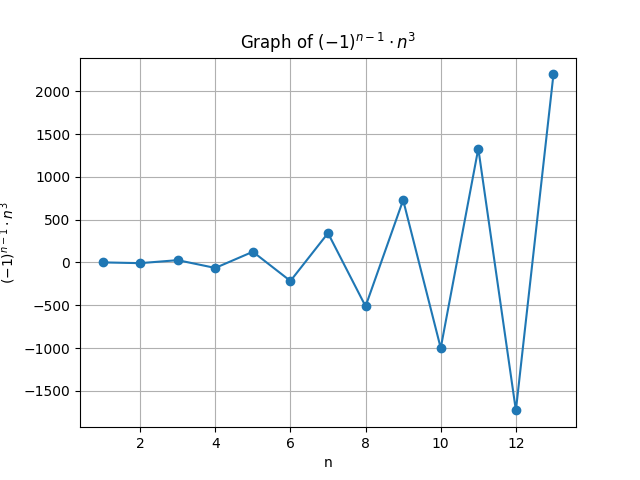
\includegraphics[scale=0.8]{assignments/digital1/graphs/graph1.png}

\end{document}
